\documentclass[10pt,a4paper]{article}
\usepackage[utf8]{inputenc}
\usepackage[T1]{fontenc}
\usepackage{lmodern}
\usepackage{textcomp}
\renewcommand{\familydefault}{\sfdefault}
\usepackage[a4paper,left=2.1cm,right=2.1cm,top=2.2cm,bottom=2.4cm]{geometry}
\usepackage{amsmath}
\usepackage[table]{xcolor}
\usepackage{graphicx}
\usepackage{tabularx}
\usepackage{array}
\usepackage{enumitem}
\usepackage{titlesec}
\usepackage{needspace}
\usepackage{fancyhdr}
\usepackage[most]{tcolorbox}
\usepackage{tikz}
\usetikzlibrary{arrows.meta,positioning,calc}
\usepackage{xurl}
\usepackage[hidelinks]{hyperref}

% ------------------------------------------------------------- couleurs
\definecolor{secblue}{HTML}{2F5F8F}
\definecolor{subpurple}{HTML}{5A4FA6}
\definecolor{rulecol}{HTML}{C9D9EA}
\definecolor{fblue}{HTML}{DCE9F7}
\definecolor{fpurple}{HTML}{E6E3F5}
\definecolor{fgreen}{HTML}{DDF0E6}
\definecolor{fyellow}{HTML}{FCF2D3}
\definecolor{fpeach}{HTML}{FBE2D9}
\definecolor{fpink}{HTML}{F7DDE6}
\definecolor{fgray}{HTML}{EFEDEA}
\definecolor{rowgray}{HTML}{F2F1EE}
\definecolor{tgreen}{HTML}{2E7D5B}
\definecolor{tyellow}{HTML}{9A7414}
\definecolor{tpeach}{HTML}{B8573A}
\definecolor{tblue}{HTML}{2F5F8F}
\definecolor{tpurple}{HTML}{5A4FA6}
\definecolor{arrowcol}{HTML}{555555}

% ------------------------------------------------------------- mise en page
\setlength{\parindent}{0pt}
\setlength{\parskip}{0.45em}
\renewcommand{\arraystretch}{1.25}
\titleformat{\section}{\needspace{14\baselineskip}\Large\bfseries\color{secblue}}{\thesection.}{0.5em}{}[{\color{rulecol}\titlerule[0.8pt]}]
\titleformat{\subsection}{\needspace{8\baselineskip}\normalsize\bfseries\color{subpurple}}{\thesubsection}{0.6em}{}
\titlespacing*{\section}{0pt}{1.6em}{0.8em}
\titlespacing*{\subsection}{0pt}{1.2em}{0.5em}

\pagestyle{fancy}
\fancyhf{}
\renewcommand{\headrulewidth}{0pt}
\lfoot{\small Captain Energy -- TSYP14 Technical Challenge}
\rfoot{\small\thepage}

% boîte à titre en onglet : {fond}{couleur du titre}{titre}
\newtcolorbox{tbox}[3]{enhanced, colback=#1, colframe=#1,
  boxrule=0pt, arc=3mm, left=3mm, right=3mm, top=4.5mm, bottom=2mm,
  fonttitle=\bfseries\small, coltitle=#2, title={#3},
  attach boxed title to top left={xshift=3mm, yshift=-2.6mm},
  boxed title style={colback=white, colframe=#1!80!gray, boxrule=0.4pt, arc=2mm},
  before skip=4mm, after skip=3mm}

% pastille de numéro pour les étapes
\newcommand{\badge}[1]{{\setlength{\fboxsep}{2.2pt}\colorbox{fpurple}{\small\bfseries\color{secblue}#1}}}
\newlist{steps}{enumerate}{1}
\setlist[steps]{label=\badge{\arabic*}, leftmargin=1.9em, itemsep=0.35em}
\setlist[itemize]{itemsep=0.2em}

% figures reprises du document d'origine (vectorielles)
\newcommand{\figorig}[2]{\begin{center}\includegraphics[page=#1,viewport=#2,clip]{orig.pdf}\end{center}}
\newcommand{\figorigw}[2]{\begin{center}\includegraphics[page=#1,viewport=#2,clip,width=\linewidth]{orig.pdf}\end{center}}

\newcolumntype{L}{>{\raggedright\arraybackslash}X}
\newcolumntype{P}[1]{>{\raggedright\arraybackslash}p{#1}}
\newcolumntype{Q}[1]{>{\raggedright\arraybackslash\bfseries}p{#1}}

\begin{document}

% ================================================================ TITRE
\begin{tcolorbox}[enhanced, colback=fblue, colframe=fblue, arc=4mm, boxrule=0pt, left=5mm, right=5mm, top=4mm, bottom=4mm]
{\fontsize{22}{26}\selectfont\bfseries\color{secblue} Captain Energy (Edge Energy Manager)}\par\vspace{2mm}
{\large\color{subpurple} Boîtier intelligent de protection et de secours électrique\\ pour les frigos et appareils des petits commerces}\par\vspace{2mm}
{\small\color{gray!70!black} TSYP14 Technical Challenge -- Edge AI \& IoT for Resilient Smart Infrastructure}
\end{tcolorbox}

\begin{tbox}{fpurple}{tpurple}{Le projet en 30 secondes}
L'été, en Tunisie, les \textbf{coupures de courant} sont fréquentes, et le courant revient souvent \textbf{brusquement}, parfois en \textbf{coupant et revenant plusieurs fois en une ou deux minutes}. Ces variations \textbf{abîment le moteur (compresseur) des frigos} et font perdre la marchandise des bouchers, épiciers, vendeurs de volaille ou pharmacies.

Notre boîtier se branche \textbf{une seule fois}, entre l'arrivée STEG et les appareils, puis \textbf{se gère tout seul}~:
\begin{enumerate}[nosep, leftmargin=2em]
  \item il \textbf{protège les appareils} contre les sous-tensions et les surtensions~;
  \item il \textbf{protège contre les retours brusques et les coupures répétées}~;
  \item il \textbf{bascule automatiquement sur batterie} en donnant la priorité à la marchandise du frigo~;
  \item son \textbf{intelligence embarquée} apprend comment le frigo se réchauffe, calcule l'autonomie et le \textbf{temps de sécurité des aliments}, \textbf{prévoit les coupures} et décide quels appareils garder allumés.
\end{enumerate}
Aucun bouton à utiliser au quotidien~: c'est pensé aussi pour des utilisateurs qui ne savent pas lire.
\end{tbox}

% ================================================================ 1
\section{Le problème}

\subsection{Les coupures en Tunisie}
Pendant les fortes chaleurs, la consommation (surtout la climatisation) met le réseau sous pression. La STEG annonce alors des \textbf{coupures programmées} (travaux de maintenance) et des \textbf{coupures tournantes} (délestage), et précise souvent que le courant peut être \textbf{rétabli sans préavis}. À l'été 2026, des délestages ont touché le Grand Tunis, Nabeul, Sousse, Sfax, Gabès et d'autres régions, souvent entre 17~h et 22~h, avec des coupures pouvant durer \textbf{jusqu'à deux heures}. À cela s'ajoutent les coupures imprévues (pannes).

\subsection{Pourquoi le frigo s'abîme}
\rowcolors{2}{white}{rowgray}
\begin{tabularx}{\linewidth}{Q{3.6cm}L}
\rowcolor{fpeach} Situation & \mdseries Ce qui arrive au moteur du frigo \\
Baisse de tension & Le compresseur tire plus de courant pour compenser~: il chauffe et son bobinage s'use. \\
Retour brusque du courant & Le compresseur redémarre alors que le gaz est encore sous pression~: il force, tire un très gros courant de démarrage et peut griller. \\
Coupures répétées (1 à 2 min) & Le courant revient, recoupe, revient\ldots{} Chaque retour est un nouveau choc. C'est le cas le plus destructeur. \\
Surtension & Les pics de tension au retour du courant endommagent l'électronique. \\
\end{tabularx}

Et pendant la coupure elle-même, \textbf{personne ne sait combien de temps la marchandise reste sûre}.

\subsection{Ce qui existe déjà et ses limites}
\rowcolors{2}{white}{rowgray}
\begin{tabularx}{\linewidth}{Q{3.4cm}LL}
\rowcolor{fblue} Solution & \mdseries Ce qu'elle fait & \mdseries Ce qui manque \\
Protecteur de tension & Coupe les appareils en sous- ou surtension, avec un délai de redémarrage réglé à la main. & Pas de secours~: pendant la coupure, le frigo s'arrête. Réglages par boutons. \\
Onduleur / batterie classique & Prend le relais pendant la coupure. & Alimente tout en même temps, se vide vite, aucune priorité, aucune protection du compresseur au retour, aucune estimation du temps de sécurité des aliments. \\
\rowcolor{fgreen} \color{tgreen}Notre boîtier & \color{tgreen}Protection + secours + priorités + intelligence, dans un seul boîtier. & \color{tgreen}Rien à régler au quotidien~: il se gère tout seul. \\
\end{tabularx}

% ================================================================ 2
\section{Notre solution : les 4 fonctions}

\begin{tcbraster}[raster columns=2, raster equal height=rows, raster column skip=4mm, raster row skip=5mm]
\begin{tbox}{fgreen}{tgreen}{1. Protection sous / surtension}
Si la tension STEG est trop basse ou trop haute, le boîtier \textbf{déconnecte les appareils du réseau} et les passe sur batterie \textbf{avant} que le moteur souffre.
\end{tbox}
\begin{tbox}{fyellow}{tyellow}{2. Protection des retours et coupures répétées}
Au retour du courant, il \textbf{attend que le réseau soit stable}, impose un \textbf{délai au compresseur} et rebranche les appareils \textbf{un par un}, en douceur.
\end{tbox}
\begin{tbox}{fpeach}{tpeach}{3. Bascule sur batterie avec priorités}
En cas de coupure, il bascule en quelques millisecondes sur batterie et \textbf{coupe d'abord les appareils les moins importants}~: la marchandise du frigo est toujours protégée en premier.
\end{tbox}
\begin{tbox}{fpurple}{tpurple}{4. Intelligence embarquée}
Il \textbf{apprend comment le frigo se réchauffe}, calcule l'\textbf{autonomie} et le \textbf{temps de sécurité des aliments}, \textbf{prévoit les coupures} (annonces STEG, chaleur, tension) et décide qui garde l'énergie.
\end{tbox}
\end{tcbraster}

\begin{tbox}{fblue}{tblue}{Le principe de sécurité}
\textbf{Les règles protègent, l'IA anticipe.} Tout ce qui protège le matériel (seuils, délais) repose sur des règles simples et sur un circuit électronique indépendant. L'IA sert à prévoir, estimer et optimiser.
\end{tbox}

% ================================================================ 3
\section{Comment ça marche}

\subsection{Les 4 états du boîtier}
\figorig{2}{70 68 522 258}

\subsection{Scénario d'une coupure, pas à pas}
\begin{steps}
  \item \textbf{Avant~:} la STEG a annoncé une coupure à 17~h, il fait 39~°C, ou la tension commence à baisser et à osciller. Le \textbf{score de risque} monte. Le boîtier calcule \textbf{quand commencer} et refroidit le frigo jusqu'au \textbf{seuil bas de la marchandise} pour «~stocker du froid~».
  \item \textbf{Coupure~:} le boîtier bascule sur batterie en quelques millisecondes. Le frigo ne s'en rend pas compte.
  \item \textbf{Pendant~:} il compare le temps de sécurité de la marchandise, l'autonomie de la batterie et la durée de coupure attendue. Il peut \textbf{éteindre le moteur du frigo si le froid stocké suffit}, et ne coupe le routeur, les lumières ou la clim que si nécessaire. La LED passe à l'orange, un message vocal et une alerte préviennent l'utilisateur.
  \item \textbf{Le courant revient, recoupe, revient\ldots} Les appareils restent sur batterie~: le moteur \textbf{ne voit aucune de ces coupures}. Le boîtier attend que le réseau soit stable.
  \item \textbf{Retour~:} il rebranche le frigo avec un démarrage doux, puis les autres appareils avec quelques secondes d'écart. La batterie recommence à se charger et la \textbf{durée de la coupure est enregistrée} pour mieux prévoir la suivante.
\end{steps}

% ================================================================ 4
\subsection{La chaîne complète : capteurs $\rightarrow$ IA $\rightarrow$ décision $\rightarrow$ action}
Le cahier des charges demande la chaîne \textbf{Sensing $\rightarrow$ Edge Processing $\rightarrow$ Connectivity $\rightarrow$ Response / Action}. Chaque capteur du boîtier alimente au moins une décision prise sur place.

\rowcolors{2}{white}{rowgray}
\begin{tabularx}{\linewidth}{Q{2.9cm}P{3.6cm}LP{3.2cm}}
\rowcolor{fgreen} Capteur & \mdseries Ce qu'il mesure & \mdseries Ce qui l'utilise (sur l'ESP32) & \mdseries Action qui en découle \\
INA219 n°1 & Tension et courant STEG & IA n°1 (état du réseau), score de risque & Bascule sur batterie avant la coupure \\
INA219 n°2 & Tension et courant de la batterie & IA n°2 (niveau de charge, autonomie) & Délestage des appareils \\
DS18B20 -- air du frigo & Température de l'air dans le frigo & Thermostat, \textbf{détection de la porte}, IA n°3 & Moteur du frigo allumé / éteint \\
DS18B20 -- magasin & Température de l'air autour du frigo & IA n°3 ($k$), consommation du frigo, règle de la clim & Pré-refroidissement, cycles de la clim \\
$T_{\text{produit}}$ \textit{(simulée dans le prototype)} & Température de la marchandise & IA n°3 (temps de sécurité), cible du pré-refroidissement & Alerte «~vendre ou déplacer avant HH:MM~» \\
Porte \textit{(sans capteur)} & Déduite des 2 sondes~: l'air monte vite et dépasse le produit & IA n°3 (ouvertures/h, apprentissage propre de $k$) & Délestage plus tôt si la porte s'ouvre souvent \\
LM393 + diviseur \textit{(version produit)} & Tension STEG, en matériel & Rien~: il agit seul & Bascule sur batterie même si l'ESP32 est planté \\
\end{tabularx}

\textbf{Connectivité~:} MQTT vers le PC (annonces STEG, météo) et vers le téléphone du propriétaire (alertes). Les décisions ne dépendent jamais d'Internet.

\section{Protection de la tension et des retours de courant}

\subsection{Les seuils}
\rowcolors{2}{white}{rowgray}
\begin{tabularx}{\linewidth}{Q{4.6cm}LL}
\rowcolor{fgreen} Seuil & \mdseries Vrai réseau (230 V) & \mdseries Prototype (12 V) \\
Sous-tension~: on passe sur batterie & $< 200$ V & $< 10{,}4$ V \\
Surtension~: on passe sur batterie & $> 255$ V & $> 13{,}3$ V \\
Retour accepté (zone «~normale~») & entre 207 et 250 V & entre 10,8 et 13,0 V \\
\end{tabularx}

{\small La zone de retour est plus étroite que les seuils de coupure (c'est une \textbf{hystérésis})~: le boîtier ne bascule pas sans arrêt quand la tension hésite autour d'un seuil.}

\subsection{Les règles anti-retours brusques et anti-coupures répétées}
\begin{tbox}{fyellow}{tyellow}{Les 5 règles de protection du matériel}
\begin{enumerate}[leftmargin=2em, itemsep=0.3em]
  \item \textbf{Attente de stabilité~:} au retour du courant, la tension doit rester correcte pendant \textbf{2 minutes} avant de rebrancher quoi que ce soit.
  \item \textbf{Chrono remis à zéro~:} si le courant recoupe ou sort de la zone normale pendant l'attente, on recommence l'attente depuis le début.
  \item \textbf{Réseau instable~:} si le boîtier compte \textbf{3 coupures ou plus en 2 minutes}, il classe le réseau comme «~instable~» et allonge l'attente à \textbf{5 minutes}.
  \item \textbf{Délai du compresseur~:} si le frigo s'est arrêté (batterie vide), il doit rester éteint \textbf{au moins 3 minutes} avant de redémarrer, le temps que la pression du gaz retombe.
  \item \textbf{Retour échelonné et doux~:} les appareils sont rebranchés \textbf{un par un} (frigo d'abord, environ 10 secondes d'écart), et le moteur du frigo démarre \textbf{progressivement} (PWM).
\end{enumerate}
\end{tbox}

\subsection{Deux niveaux de protection}
\rowcolors{2}{white}{rowgray}
\begin{tabularx}{\linewidth}{Q{3.6cm}LP{2.8cm}}
\rowcolor{fpurple} Niveau & \mdseries Rôle & \mdseries Vitesse \\
Circuit matériel (comparateur LM393, \textit{version produit, non câblé sur la maquette}) & Bascule sur batterie si la tension sort de la fenêtre normale, \textbf{même si l'ESP32 est planté}. & quelques microsecondes \\
ESP32 + IA & Anticipation, priorités, attente de stabilité, retour progressif, alertes. & millisecondes à minutes \\
\end{tabularx}

% ================================================================ 5
\section{Bascule sur batterie, priorités et intelligence}

\subsection{Les priorités}
\rowcolors{2}{white}{rowgray}
\begin{tabularx}{\linewidth}{Q{1.4cm}P{2.8cm}L}
\rowcolor{fpeach} Priorité & \mdseries Appareil & \mdseries Règle \\
P1 & Frigo & La marchandise passe toujours en premier (le moteur peut être éteint si le froid stocké suffit, voir 5.9). \\
P2 & Climatiseur & Gardé si la chaleur est forte \textbf{et} si la batterie le permet (cycles courts). \\
P3 & Lumières & Coupées si l'autonomie devient insuffisante. \\
P4 & Routeur / autres & Coupés en premier. \\
\end{tabularx}

Les priorités ne sont \textbf{pas figées}~: elles changent selon la situation.

\rowcolors{2}{white}{rowgray}
\begin{tabularx}{\linewidth}{Q{5cm}L}
\rowcolor{fpurple} Situation détectée & \mdseries Décision \\
Coupure annoncée à 17 h & Pré-refroidissement lancé à l'heure \textbf{calculée} (section 5.8), batterie chargée au maximum. \\
Frigo plein et 38~°C dehors & Frigo en priorité absolue~; clim coupée sauf si la batterie est haute. \\
Frigo presque vide & Sa priorité baisse~: la clim ou les lumières peuvent rester allumées. \\
Clinique et plus de 35~°C & Clim par cycles courts (10 min allumée, 20 min éteinte) si la batterie le permet. \\
Batterie sous 20~\% & Seul le frigo reste allumé. \\
Autonomie $<$ durée de coupure attendue & Délestage plus tôt pour tenir jusqu'au retour du courant, et alerte précoce. \\
\end{tabularx}

\subsection{Où se trouve l'IA}
\begin{center}
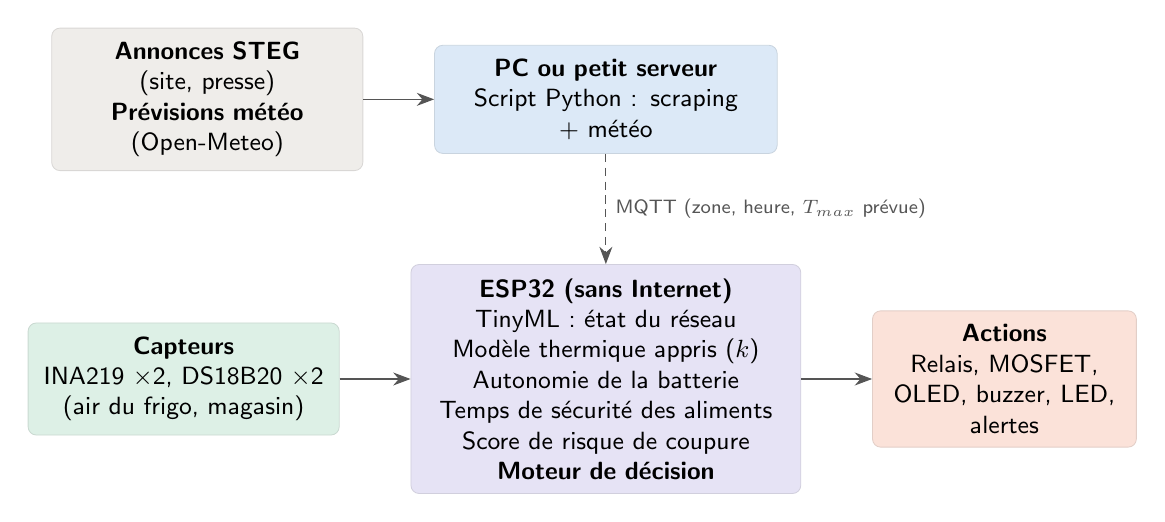
\begin{tikzpicture}[
  box/.style={rounded corners=3pt, align=center, font=\small, inner sep=5pt, draw=#1!80!gray, fill=#1, line width=0.3pt},
  >={Stealth[length=2.2mm]}]
  \node[box=fgray, text width=3.6cm] (web) {\textbf{Annonces STEG}\\(site, presse)\\\textbf{Prévisions météo}\\(Open-Meteo)};
  \node[box=fblue, text width=4cm, right=9mm of web] (pc) {\textbf{PC ou petit serveur}\\Script Python~: scraping\\+ météo};
  \node[box=fpurple, text width=4.6cm, below=14mm of pc] (esp) {\textbf{ESP32 (sans Internet)}\\TinyML~: état du réseau\\Modèle thermique appris ($k$)\\Autonomie de la batterie\\Temps de sécurité des aliments\\Score de risque de coupure\\\textbf{Moteur de décision}};
  \node[box=fgreen, text width=3.6cm, left=9mm of esp] (cap) {\textbf{Capteurs}\\INA219 $\times$2, DS18B20 $\times$2\\(air du frigo, magasin)};
  \node[box=fpeach, text width=3cm, right=9mm of esp] (act) {\textbf{Actions}\\Relais, MOSFET,\\OLED, buzzer, LED,\\alertes};
  \draw[->, arrowcol] (web) -- (pc);
  \draw[->, arrowcol, dashed, densely dashed] (pc) -- node[right, font=\scriptsize]{MQTT (zone, heure, $T_{max}$ prévue)} (esp);
  \draw[->, arrowcol] (cap) -- (esp);
  \draw[->, arrowcol] (esp) -- (act);
\end{tikzpicture}
\end{center}

Le web scraping se fait sur un PC car l'ESP32 n'a pas assez de mémoire pour lire des pages web. C'est un \textbf{bonus}~: les annonces ne couvrent que les coupures prévues. Les capteurs restent la détection principale, et le boîtier fonctionne entièrement sans Internet.

\subsection{IA n°1 : reconnaître l'état du réseau}
Toutes les secondes, l'ESP32 prend une fenêtre de mesures de tension (INA219 n°1) et en extrait quelques caractéristiques~: moyenne, minimum, écart-type, nombre de creux. Un petit modèle \textbf{TinyML} (quantifié en int8) classe la situation en \textbf{normal}, \textbf{instable}, \textbf{baisse} ou \textbf{coupure}. Il permet de basculer \textbf{avant} la coupure quand la tension montre des signes de faiblesse. Les seuils de sécurité, eux, restent des règles fixes.

\subsection{IA n°2 : niveau de batterie et autonomie}
\textbf{Étape 1 -- Le niveau de charge (SoC).} L'INA219 n°2 mesure le courant qui sort de la batterie. On additionne ce courant dans le temps (\textbf{comptage de charge})~:
\[ \mathrm{SoC}(t) = \mathrm{SoC}(t_0) - \frac{1}{C_n}\int_{t_0}^{t} I(\tau)\,d\tau \]
et on corrige régulièrement avec la tension au repos de la batterie~:
\begin{center}
\rowcolors{1}{fgreen}{rowgray}
\begin{tabular}{rccccc}
Tension au repos (V) & 12,7 & 12,5 & 12,2 & 12,1 & 11,8 \\
Niveau de charge & 100~\% & 80~\% & 60~\% & 50~\% & 30~\% \\
\end{tabular}\\[1mm]
{\small (valeurs approximatives pour une batterie plomb 12~V)}
\end{center}

\textbf{Étape 2 -- L'énergie utilisable.} On ne vide jamais complètement une batterie~: on garde une \textbf{réserve} $\mathrm{SoC}_{\min}$. Pour une batterie \textbf{plomb} (produit final), on ne descend pas sous 50~\%~: au-delà, elle s'use très vite. Pour les cellules \textbf{Li-ion} de la maquette, la réserve est seulement de 10~\% (environ 3,2 V par cellule)~:
\[ E_{\text{utile}} = (\mathrm{SoC} - \mathrm{SoC}_{\min}) \times C_n \times U_n \]

\textbf{Étape 3 -- L'autonomie.}
\[ t_{\text{autonomie}} = \frac{E_{\text{utile}}}{P_{\text{consommée}}} \]

\begin{tbox}{fgreen}{tgreen}{Exemple de calcul (batterie 12 V -- 7 Ah, pleine)}
$E_{\text{utile}} = (1 - 0{,}5) \times 7\ \text{Ah} \times 12\ \text{V} = 42$ Wh.
\begin{itemize}[nosep]
  \item Tout allumé (frigo 12 W + ventilateur 6 W + LED 5 W + routeur 6 W = 29 W)~: $42/29 \approx$ \textbf{1 h 27}.
  \item Frigo seul (12 W)~: $42/12 =$ \textbf{3 h 30}.
\end{itemize}
Les priorités font passer l'autonomie du frigo de 1 h 27 à 3 h 30 avec la même batterie. (Avec le module Peltier de la maquette, qui consomme plus, ces durées seront plus courtes~: les vraies valeurs sont mesurées.)
\end{tbox}

\begin{tbox}{fblue}{tblue}{Même calcul pour la maquette (pack 3S Li-ion 18650, 1,5 Ah, plein)}
$E_{\text{utile}} = (1 - 0{,}1) \times 1{,}5\ \text{Ah} \times 11{,}1\ \text{V} \approx 15$ Wh. Peltier (3 A $\times$ 11,4 V $\approx$ 34 W)~: $15/34 \approx$ \textbf{26 minutes}. À moitié chargé (50~\%)~: $(0{,}5 - 0{,}1) \times 1{,}5 \times 11{,}1 \approx 6{,}7$ Wh, soit \textbf{environ 12 minutes}.
\end{tbox}

\textbf{Où est l'IA~?} La consommation du frigo n'est pas constante~: le compresseur tourne plus souvent quand il fait chaud ou quand le frigo est plein. Un petit modèle de \textbf{régression} apprend la consommation moyenne à partir de la température extérieure, de la température du frigo et de son remplissage. L'autonomie estimée est donc beaucoup plus juste qu'une simple division.

\subsection{IA n°3 : modèle thermique appris du frigo}
\textbf{Le problème d'une formule simple.} La formule $t_{\text{sûr}} = (T_{\max} - T_{\text{actuelle}})/(dT/dt)$ a besoin de la vitesse de montée $dT/dt$. Or, au tout début d'une coupure, le frigo vient de s'arrêter~: on ne connaît pas encore cette vitesse. Et elle change si la chaleur extérieure change pendant la coupure.

\textbf{La solution~: apprendre une constante propre à chaque frigo.} On utilise la loi de refroidissement de Newton~:
\[ \frac{dT}{dt} = k\,\bigl(T_{\text{amb}} - T\bigr) \]
où $T$ est la température dans le frigo et $T_{\text{amb}}$ la température de l'air du magasin, \textbf{autour du frigo}.
Le coefficient $k$ résume tout ce qui fait qu'un frigo se réchauffe plus ou moins vite~: isolation, taille, \textbf{quantité de marchandise} (la masse froide), état du joint de porte. On ne mesure rien de tout cela à la main~: \textbf{l'ESP32 apprend $k$ tout seul}.

\textbf{Quand l'apprend-il~?} En temps normal, le moteur du frigo s'arrête et redémarre plusieurs fois par heure (cycles du thermostat). Pendant chaque arrêt, porte fermée, l'ESP32 enregistre des couples $x_i = T_{\text{amb},i} - T_i$ et $y_i = \Delta T_i / \Delta t$, et met à jour $k$ par \textbf{moindres carrés avec oubli}~:
\[ S_{xy} \leftarrow \lambda S_{xy} + x_i y_i, \qquad S_{xx} \leftarrow \lambda S_{xx} + x_i^2, \qquad \hat{k} = \frac{S_{xy}}{S_{xx}} \]
Le facteur d'oubli $\lambda \approx 0{,}98$ donne plus de poids aux mesures récentes~: si le commerçant remplit ou vide son frigo, $k$ s'adapte en quelques cycles. Ce calcul ne demande que deux variables en mémoire~: il tourne sans difficulté sur l'ESP32, sans Internet.

\textbf{Le temps de sécurité dès la première seconde de la coupure.} Avec $k$ déjà connu~:
\[ t_{\text{sûr}} = -\frac{1}{k}\,\ln\!\left(\frac{T_{\text{amb}} - T_{\max}}{T_{\text{amb}} - T_{\text{produit}}}\right) \qquad (T_{\text{produit}} < T_{\max} < T_{\text{amb}}) \]

\begin{tbox}{fgreen}{tgreen}{Exemple illustratif ($k = 0{,}02$ h$^{-1}$, $T_{\text{amb}} = 35$ °C, $T_{\max} = 4$ °C)}
\begin{itemize}[nosep]
  \item Marchandise à 3~°C au début de la coupure~: $t_{\text{sûr}} \approx$ \textbf{1 h 35}.
  \item Marchandise pré-refroidie à 1~°C~: $t_{\text{sûr}} \approx$ \textbf{4 h 37}.
\end{itemize}
Deux degrés de pré-refroidissement font presque \textbf{tripler} le temps de sécurité. (Valeur de $k$ choisie pour l'exemple~; la vraie valeur est mesurée sur la maquette.)
\end{tbox}

\textbf{Honnêtement.} Entre 0 et 5~°C, la courbe est presque une droite~: la formule de Newton ne change pas beaucoup le résultat. Son vrai intérêt est ailleurs~: $k$ est \textbf{connu avant la coupure}, il sert à planifier le pré-refroidissement, il tient compte d'une chaleur extérieure qui monte pendant l'après-midi, et il indique si le frigo est \textbf{plein} ($k$ petit) ou \textbf{vide} ($k$ grand).

\textbf{Un réseau entraîné sur toutes les coupures possibles.} Newton seul ignore les ouvertures de porte, l'air plus chaud que la marchandise et le magasin qui se réchauffe. Le boîtier utilise donc un petit réseau de neurones (7 entrées, 16 neurones, poids int8, 129 octets) qui donne le temps de sécurité \textbf{dès la première seconde de la coupure}, à partir de $T_{\text{produit}}$, $T_{\text{air}}$, $T_{\text{amb}}$, $T_{\max}$, $k$, du nombre d'ouvertures de porte par heure et du résultat de Newton. Il est entraîné sur \textbf{40\,000 coupures simulées} par un modèle physique (air + marchandise), qui couvrent tous les cas~: petite boîte ou vrai frigo, vide ou plein, $T_{\max}$ de 2 à 18~°C, magasin de 18 à 42~°C qui peut se réchauffer pendant la coupure, 0 à 20 ouvertures de porte par heure, marchandise déjà trop chaude.

\rowcolors{2}{white}{rowgray}
\begin{tabularx}{\linewidth}{Q{5.2cm}P{3.2cm}L}
\rowcolor{fgreen} Sur 8\,000 coupures de test jamais vues & \mdseries Erreur relative médiane & \mdseries Temps surestimé de plus de 10~\% \\
Formule de Newton seule & 33~\% & 25,6~\% des cas \\
Réseau int8 (ESP32) & \textbf{23~\%} & 38,9~\% des cas \\
Réseau $\times$ marge de prudence 0,51 (utilisé) & 50~\% & \textbf{3,3~\%} des cas \\
\end{tabularx}
Surestimer le temps de sécurité est dangereux, le sous-estimer coûte seulement un peu de batterie~: le boîtier applique donc une marge qui rend 95~\% des prédictions prudentes.

\textbf{Température de la marchandise.} Le prototype n'a pas de sonde dans la marchandise~: $T_{\text{produit}}$ est une \textbf{donnée simulée} (elle suit l'air avec un retard de 15 minutes, comme une marchandise qui a de la masse). Une 3e sonde DS18B20 plongée dans une bouteille d'eau au milieu de la marchandise la remplacera dans le produit final, sans changer le réseau.

\textbf{La porte, sans capteur de porte.} Quand la porte s'ouvre, l'air chaud du magasin entre~: la sonde d'air monte vite (au moins 0,3~°C en 10 s) et dépasse la marchandise, alors que porte fermée elle ne peut monter que lentement. Le boîtier en déduit les ouvertures, les compte, les exclut de l'apprentissage de $k$ et les donne au réseau. Testé sur une boîte simulée~: ouvertures de 10 à 45 s toutes détectées, aucune fausse alerte en 6 heures.

\subsection{Profils de marchandise : seuil bas et seuil haut}
Chaque marchandise a une température maximale (au-dessus, elle n'est plus sûre) \textbf{et} une température minimale (en dessous, elle s'abîme ou gèle). Le pré-refroidissement descend jusqu'au seuil bas, \textbf{jamais en dessous}.

\rowcolors{2}{white}{rowgray}
\begin{tabularx}{\linewidth}{Q{4.4cm}P{1.4cm}P{1.4cm}L}
\rowcolor{fblue} Profil & \mdseries $T_{\min}$ & \mdseries $T_{\max}$ & \mdseries Pourquoi le seuil bas \\
Viande, volaille fraîche & 0~°C & 4~°C & Proche du gel, on peut descendre bas. \\
Produits laitiers & 1~°C & 4~°C & Éviter le gel. \\
Médicaments (insuline, vaccins) & 2~°C & 8~°C & \textbf{Ne doivent jamais geler.} \\
Fruits et légumes & 4~°C & 10~°C & Certains (tomates, concombres) s'abîment au froid. \\
\end{tabularx}

{\small Valeurs indicatives à vérifier avec la réglementation en vigueur et, pour les médicaments, avec la notice du fabricant.}

Si le frigo contient plusieurs profils, le boîtier prend les seuils les plus stricts~: le plus haut des $T_{\min}$ et le plus bas des $T_{\max}$.

\textbf{Comment choisir le profil sans bouton~?} Le profil est choisi \textbf{une seule fois à l'installation} par l'installateur (page web locale de l'ESP32 ou message MQTT). En option, un lecteur RFID RC522 et des \textbf{badges illustrés} (dessin d'un poulet, d'une boîte de médicament\ldots) permettent au commerçant de changer de profil en approchant un badge, sans rien lire ni écrire.

\subsection{Prévoir le risque et la durée de la coupure}
Le boîtier combine quatre signaux en un \textbf{score de risque} $R$ compris entre 0 et 1~:
\[ R = 0{,}5\,A + 0{,}2\,H + 0{,}1\,P + 0{,}2\,I \]

\rowcolors{2}{white}{rowgray}
\begin{tabularx}{\linewidth}{Q{0.9cm}P{5cm}L}
\rowcolor{fpurple} Signal & \mdseries Source & \mdseries Valeur \\
$A$ & Annonce STEG (script Python sur PC, via MQTT~; ou commande \texttt{annonce=} pour la démo) & 1 si une coupure est annoncée pour la zone dans l'heure qui vient, sinon 0. \\
$H$ & Prévision météo (API Open-Meteo, même script)~; \textbf{sans prévision~: température mesurée du magasin} (DS18B20 du magasin) & 0 à 32~°C, 1 à 40~°C, linéaire entre les deux. \\
$P$ & Heure donnée par Internet (NTP)~; l'ESP32 n'a pas d'horloge propre & 1 entre 17~h et 22~h en été (horaires fréquents des délestages de 2026), sinon 0. Sans Internet~: 0, sauf avec un module horloge DS3231 (option). \\
$I$ & IA n°1, sur l'ESP32 & Probabilité «~instable~» ou «~baisse~» donnée par le modèle TinyML. \\
\end{tabularx}

Si $R \geq 0{,}5$, le boîtier lance le pré-refroidissement~: une annonce STEG suffit à elle seule.

\textbf{Sans annonce STEG} (pas d'Internet, ou aucune coupure annoncée), $A$ n'existe pas. Le boîtier divise alors les autres signaux par 0,5 (leur poids total) pour que le score puisse encore atteindre le seuil~; sans prévision météo, $H$ vient de la température mesurée du magasin~:
\[ R_{\text{sans annonce}} = \frac{0{,}2\,H + 0{,}1\,P + 0{,}2\,I}{0{,}5} = 0{,}4\,H + 0{,}2\,P + 0{,}4\,I \]
Les coupures non annoncées (pannes) restent ainsi prévisibles, avec ou sans Internet. Exemples testés~: sans Internet, magasin à 38~°C et réseau instable ($I = 0{,}7$) donnent $R = 0{,}58$~; avec Internet sans annonce, 39~°C prévus et réseau instable donnent $R = 0{,}63$~: dans les deux cas le boîtier pré-refroidit. Magasin à 25~°C et réseau calme~: $R$ reste sous 0,5.

Exemple de message MQTT envoyé par le script (les heures sont en secondes depuis 1970, le format que l'ESP32 compare à son horloge~; ici le 20/07/2026 de 17~h à 22~h)~:\\[1mm]\hspace*{1em}\texttt{\small \{"zone":"Ariana","debut":1784563200,"fin":1784581200,"tmax\_prevue":39\}}

\textbf{Durée de coupure attendue.} Si la STEG annonce une fenêtre (17~h -- 22~h), le boîtier l'utilise. Sinon, il part de \textbf{2 h} (durée annoncée pour les délestages de l'été 2026), puis remplace cette valeur par la moyenne des coupures qu'il a lui-même mesurées dans sa zone.

\textbf{Honnêtement.} Les poids du score sont fixés à la main pour le prototype, faute d'historique de coupures réel. Une fois déployé, chaque boîtier enregistre ses coupures~: ces données permettront d'entraîner un vrai modèle de prévision.

\subsection{Pré-refroidissement calculé, pas fixe}
Au lieu de commencer toujours 30 minutes avant, le boîtier calcule l'heure de départ~:
\[ T_{\text{cible}} = T_{\min,\text{profil}} + 1\ \text{°C}, \qquad t_{\text{départ}} = t_{\text{coupure}} - \frac{T_{\text{produit}} - T_{\text{cible}}}{v_f} - \text{marge} \]
où $v_f$ est la vitesse de refroidissement du frigo (°C par minute quand le moteur tourne), apprise de la même façon que $k$. Un frigo plein met plus longtemps à descendre~: il commence plus tôt.

\subsection{Le moteur de décision}
Il compare en permanence le \textbf{temps de sécurité de la marchandise}, l'\textbf{autonomie de la batterie}, la \textbf{chaleur extérieure} et la \textbf{durée de coupure attendue}. Il donne un score à chaque appareil et coupe ceux qui ont le score le plus bas. Il peut être programmé avec des règles à score, ou remplacé par un petit \textbf{arbre de décision} entraîné sur des scénarios simulés.

Garder le frigo «~en premier~» ne veut pas dire le faire tourner sans arrêt~: \textbf{le froid stocké dans la marchandise est une réserve d'énergie gratuite.}

\rowcolors{2}{white}{rowgray}
\begin{tabularx}{\linewidth}{P{5.2cm}L}
\rowcolor{fpeach} \textbf{Situation} & Décision \\
$t_{\text{sûr}} > t_{\text{coupure}}$ & Moteur du frigo \textbf{éteint}~: le froid stocké suffit. Lumières et ventilateur restent allumés, le commerce fonctionne normalement. \\
$t_{\text{sûr}} < t_{\text{coupure}} < t_{\text{autonomie, frigo seul}}$ & On laisse la température monter jusqu'à $T_{\max} - 0{,}5$~°C, puis cycles courts du moteur. Les autres appareils sont coupés selon leur score. \\
$t_{\text{autonomie}} + t_{\text{sûr}} < t_{\text{coupure}}$ & La batterie ne tiendra pas~: \textbf{alerte précoce} au propriétaire avec l'heure limite. \\
Porte ouverte souvent & $k$ effectif augmente, $t_{\text{sûr}}$ baisse~: délestage plus tôt. \\
\end{tabularx}

\begin{tbox}{fblue}{tblue}{Des alertes qui disent quoi faire}
\begin{itemize}[nosep]
  \item «~Coupure. Batterie~: 3 h 10. Marchandise sûre~: 4 h 30. Lumières coupées.~»
  \item «~La batterie ne suffira pas pour cette coupure. Vendez ou déplacez la volaille avant 19 h 30.~»
  \item «~Coupure annoncée à 17 h~: refroidissement renforcé depuis 16 h 10.~»
\end{itemize}
\end{tbox}

\subsection{Pour des utilisateurs qui ne savent pas lire}
\begin{itemize}
  \item \textbf{LED de couleur~:} vert = tout va bien, orange = sur batterie, rouge = batterie presque vide ou marchandise en danger.
  \item \textbf{Buzzer} et, en option, \textbf{messages vocaux en derja} (module son DFPlayer Mini), avec les mêmes messages que ci-dessus.
  \item \textbf{Alertes sur téléphone} (Wi-Fi / MQTT) pour le propriétaire ou un proche.
  \item \textbf{Badges RFID illustrés} (option) pour changer de profil de marchandise.
  \item \textbf{Aucun bouton} à toucher au quotidien.
\end{itemize}

\subsection{Données et entraînement des modèles}
\rowcolors{2}{white}{rowgray}
\begin{tabularx}{\linewidth}{Q{4cm}L}
\rowcolor{fgreen} Modèle & \mdseries D'où viennent les données \\
IA n°1 -- état du réseau & Jeu de données créé au labo avec l'alimentation réglable~: tension normale, baisses lentes, oscillations, coupures et retours répétés. Chaque fenêtre d'une seconde est étiquetée, puis le modèle est entraîné dans Edge Impulse et exporté en int8. \\
IA n°2 -- consommation & Régression entraînée sur les mesures de l'INA219 enregistrées à différentes températures du magasin et différents remplissages du frigo. \\
IA n°3 -- temps de sécurité & $k$~: appris en ligne sur l'ESP32. Réseau~: entraîné sur 40\,000 coupures simulées (jeu de données \texttt{safety\_dataset.csv}), puis exporté en int8 et vérifié en C++. \\
Score de risque & Poids fixés à la main pour le prototype~; à réentraîner avec l'historique des coupures enregistrées. \\
\end{tabularx}

À mesurer et à présenter au jury~: \textbf{temps d'inférence}, \textbf{mémoire occupée} et \textbf{précision} sur un jeu de test.

% ================================================================ 6
\section{Le matériel nécessaire}

\begin{tbox}{fgreen}{tgreen}{La maquette réellement construite pour le concours}
Le tableau plus bas décrit la conception complète du boîtier. La maquette présentée au jury utilise un sous-ensemble, adapté au matériel disponible~:
\begin{itemize}[nosep]
  \item \textbf{«~STEG~» simulée~:} pack n°1, 3 cellules Li-ion 18650 (3,7 V, 1500 mAh) en série (9,6 à 12,6 V) + potentiomètre 10 k$\Omega$, mesuré par l'INA219. Tourner le potentiomètre = baisse ou instabilité~; débrancher = coupure.
  \item \textbf{Batterie de secours~:} pack n°2, 3 cellules Li-ion 18650 (3,7 V, 1500 mAh) en série, soit 1,5 Ah, fusible 5 A (environ 20 à 25 minutes de Peltier). Son niveau est calculé à partir de sa tension et du courant mesurés par l'INA219 n°2.
  \item \textbf{Froid~:} Peltier \textbf{TEC1-12704} (environ 3 A) dans une boîte en polystyrène, commandé par un \textbf{module relais 2 canaux 5 V} (canal 1, contact NO), ventilateur toujours allumé côté chaud.
  \item \textbf{Mesures~:} \textbf{2 INA219} (n°1~: tension STEG~; n°2~: tension et courant du pack n°2), \textbf{2 DS18B20} (air de la boîte, air du magasin), \textbf{pas de contact de porte} (porte déduite des températures). La température de la marchandise est une \textbf{donnée simulée}.
  \item \textbf{Appareils simulés~:} 2 LED (clim, lumières)~; LED RGB, buzzer et écran OLED pour les alertes.
  \item \textbf{Non câblés sur la maquette (version produit)~:} comparateur LM393, MOSFET et démarrage doux, PCB.
\end{itemize}
\end{tbox}

\rowcolors{2}{white}{rowgray}
\begin{tabularx}{\linewidth}{Q{2.3cm}P{5.6cm}P{0.8cm}L}
\rowcolor{fpeach} Catégorie & \mdseries Composant & \mdseries Qté & \mdseries Rôle \\
Cerveau & ESP32 DevKit V1 & 1 & Calculs, IA, commande \\
Mesure & INA219 & 2 & Tension et courant~: STEG et batterie \\
 & DS18B20 étanche + résistance 4,7 k$\Omega$ & \textbf{2} & Air dans le frigo, air du magasin autour du frigo (une 3e sonde produit en option, produit final) \\
Protection matérielle & LM393 (double comparateur) & 1 & Fenêtre sous / surtension, indépendante de l'ESP32 \\
 & 2 potentiomètres 10 k$\Omega$, diviseur 10 k$\Omega$ / 3,3 k$\Omega$, 2 résistances 1 M$\Omega$, 1 résistance 10 k$\Omega$ & -- & Seuils, hystérésis, pull-up \\
 & Diodes 1N4148 & 2 & «~OU~» entre le comparateur et l'ESP32 \\
Commande & Module relais 4 canaux 5 V & 1 & Bascule STEG / batterie + 3 appareils \\
 & MOSFET logique IRLZ44N + résistances 100 $\Omega$ et 10 k$\Omega$ & 1 & Démarrage doux / PWM du frigo \\
Froid (maquette) & \textbf{Module Peltier TEC1-12703 + 2 dissipateurs + ventilateur, pâte thermique, boîte en polystyrène} & 1 & \textbf{Vraie source de froid}, commandée par le MOSFET Q1 \\
Protections & Fusibles rapides 2 A et 5 A + porte-fusibles & 2 & Contre les courts-circuits \\
 & Diode TVS SMBJ15A & 1 & Contre les pics de tension \\
 & Diode Schottky SS54 (ou MOSFET P AO4407 + Zener 12 V) & 1 & Contre l'inversion de polarité \\
 & Diodes Schottky 1N5819 & 2 & Roue libre~: Peltier/moteur et ventilateur \\
 & Condensateur 1000 $\mu$F / 25 V & 1 & Rend la bascule invisible \\
Énergie & Batterie plomb 12 V -- 7 Ah & 1 & Secours \\
 & Convertisseur buck LM2596 (12 V $\rightarrow$ 5 V) & 1 & Alimente l'ESP32 et les relais \\
 & Alimentation de labo réglable & 1 & Simule la STEG (déjà au labo) \\
Interface & OLED 0,96'' I2C, buzzer, LED RGB + 3 $\times$ 220 $\Omega$ & 1 & Alertes sur place \\
 & Lecteur RFID RC522 + badges (option) & 1 & Choix du profil de marchandise sans lire \\
Démonstration & Ventilateur 12 V, ruban LED 12 V, routeur & 1 & Les autres appareils du «~magasin~» \\
\end{tabularx}

\textbf{Logiciels~:} Arduino IDE ou PlatformIO, Edge Impulse ou TensorFlow Lite Micro, Python + broker MQTT (Mosquitto), API Open-Meteo, KiCad pour la carte.

\textbf{Pourquoi un Peltier~?} Un moteur 12~V dans une glacière représente le compresseur \emph{électriquement}, mais il ne produit pas de froid~: la température ne baisserait jamais, et ni le pré-refroidissement ni le temps de sécurité ne seraient démontrables. Le Peltier, monté entre deux dissipateurs avec un ventilateur côté chaud, refroidit réellement la boîte.

\textbf{Volontairement absent~:} pas de capteur de courant par appareil (l'INA219 n°2 mesure le total, et l'ESP32 sait quels relais sont allumés), pas de chargeur dans le prototype (on charge la batterie avant la démo), pas de capteur d'humidité (il ne change aucune décision).

\begin{tbox}{fpeach}{tpeach}{Limites à respecter}
L'INA219 supporte au maximum 26~V et environ 3,2~A. Le Peltier tire environ 2 à 3~A~: avec le ventilateur, les LED et le routeur, le total peut dépasser cette limite et le fusible F1 de 2~A. Il faut \textbf{limiter le PWM du Peltier} (par exemple 60~\%) ou passer à un \textbf{INA226 avec un shunt externe}.
\end{tbox}

% ================================================================ 7
\section{Le circuit complet}

\subsection{Vue d'ensemble}
\figorigw{7}{50 380 545 662}

{\small Dans la maquette, le «~moteur frigo~» P1 est le module Peltier, sur le même MOSFET~; le bus des DS18B20 porte deux sondes (air du frigo, air du magasin)~; il n'y a pas de contact de porte.}

Note~: les GPIO de l'ESP32 commandent le MOSFET du frigo et les relais 2 à 4 (voir 7.6). La commande «~IN1~» du relais 1 vient à la fois de l'ESP32 et du comparateur LM393. Le relais passe sur batterie si \textbf{l'un ou l'autre} le demande, et ne revient sur la STEG que si \textbf{les deux} sont d'accord.

\subsection{Deux choix de sécurité importants}
\begin{itemize}
  \item \textbf{La STEG est branchée sur le contact NC (repos) du relais 1.} Si l'ESP32 plante ou n'est plus alimenté, les appareils restent sur la STEG~: le système est \textbf{sûr en cas de panne}.
  \item \textbf{L'ESP32 est alimenté par la batterie, pas par le bus.} Sinon, il s'éteindrait au moment de la coupure, juste quand il doit agir.
\end{itemize}

\subsection{Détail 1 : l'entrée STEG et l'entrée batterie}
\figorigw{8}{55 508 548 762}

\subsection{Détail 2 : le bus 12 V et le moteur du frigo}
\figorig{8}{90 340 525 478}

Le PWM fait monter la tension du moteur progressivement (de 0 à 100~\% en environ 2 secondes)~: le pic de courant au démarrage disparaît. La diode D3 protège le MOSFET (voir section 10). Une résistance de 10 k$\Omega$ entre la grille et la masse garde le moteur éteint au démarrage de l'ESP32. Le même MOSFET règle aussi la puissance du Peltier (pré-refroidissement, cycles courts).

\subsection{Détail 3 : le comparateur fenêtre LM393 (version produit)}
\figorig{8}{58 150 535 258}

Les deux sorties du LM393 sont à collecteur ouvert~: elles se relient directement entre elles. Si la tension est trop basse \textbf{ou} trop haute, la sortie tire IN1 vers la masse et le relais passe sur batterie. Les deux seuils se règlent avec deux potentiomètres de 10 k$\Omega$ alimentés en 5 V, et une résistance de 1 M$\Omega$ par comparateur ajoute l'hystérésis.

\subsection{Branchement sur l'ESP32}
\rowcolors{2}{white}{rowgray}
\begin{tabularx}{\linewidth}{LP{3.6cm}P{3.2cm}}
\rowcolor{fblue} \textbf{Composant} & Broche du composant & ESP32 \\
INA219 n°1 (0x40), INA219 n°2 (0x41, pont A0 soudé), OLED (0x3C) & SDA / SCL / VCC / GND & GPIO21 / GPIO22 / 3V3 / GND \\
2 $\times$ DS18B20 (même fil) & DQ + 4,7 k$\Omega$ vers 3V3 & GPIO4 \\
Relais 1~: bascule STEG / batterie & IN1 (via 1N4148) & GPIO26 \\
Relais 2~: climatiseur & IN2 & GPIO25 \\
Relais 3~: lumières & IN3 & GPIO33 \\
Relais 4~: routeur & IN4 & GPIO32 \\
Module relais & VCC / GND & 5 V du buck / GND \\
MOSFET du frigo (Peltier) & Grille (via 100 $\Omega$) & GPIO18 (PWM) \\
Buzzer & + & GPIO19 \\
LED RGB (via 220 $\Omega$) & R / G / B & GPIO16 / 17 / 23 \\
RC522 (option, SPI) & SDA / SCK / MOSI / MISO / RST & GPIO5 / 14 / 13 / 34 / 27 \\
Buck 5 V & OUT+ & VIN \\
\end{tabularx}

{\small Les modules relais s'activent à l'état bas~: il faut mettre ces broches à HIGH dès le démarrage dans le code, sinon les relais claquent à chaque reset. Le RC522 utilise des broches libres en SPI logiciel~; MISO est sur GPIO34, une broche en entrée seule, ce qui suffit pour une donnée reçue.}

% ================================================================ 8
\section{La démonstration devant le jury}
\begin{steps}
  \item \textbf{Fonctionnement normal~:} potentiomètre du pack «~STEG~» vers 11,5 V, LED allumées, Peltier qui refroidit. La commande \texttt{info} montre la classe de l'IA n°1, le temps d'inférence et le courant du Peltier.
  \item \textbf{L'IA anticipe la baisse~:} on tourne lentement le potentiomètre vers 10,8 V. L'IA n°1 reconnaît une «~baisse~» et le boîtier bascule \textbf{avant} le seuil de 10,4 V.
  \item \textbf{Coupures répétées~:} on débranche et rebranche le fil «~STEG~» trois fois en une minute. Les appareils restent sur batterie, le Peltier ne voit rien, le boîtier attend 5 minutes de stabilité.
  \item \textbf{Coupure annoncée~:} commande \texttt{annonce=20,2,39} (coupure dans 20 min, 39~°C prévus). Le score de risque passe au-dessus de 0,5 et le Peltier \textbf{pré-refroidit} la boîte.
  \item \textbf{Même coupure, deux décisions~:} une coupure courte annoncée (le froid stocké suffit~: Peltier éteint, lumières gardées), puis une coupure longue (délestage et alerte «~vendez ou déplacez avant HH:MM~»).
  \item \textbf{Porte ouverte~:} on ouvre le couvercle pendant une coupure~: le temps de sécurité baisse en direct.
  \item \textbf{Batterie faible~:} commande \texttt{soc=15}~: seul le frigo reste alimenté.
  \item \textbf{Panne du Peltier~:} on débranche un fil du Peltier pendant qu'il tourne~: le boîtier détecte qu'il ne consomme plus rien et envoie une alerte.
  \item \textbf{Modèle appris~:} on montre la courbe de réchauffement de la boîte et le $k$ appris par l'ESP32.
\end{steps}

{\small Le réchauffement d'une boîte prend du temps~: la courbe complète du temps de sécurité est enregistrée à l'avance et montrée accélérée, en le disant clairement au jury.}

% ================================================================ 9
\section{La carte PCB sous KiCad}
Pour montrer que le produit peut être fabriqué en série, on regroupe tout le montage sur une carte PCB dessinée dans KiCad (logiciel gratuit). L'ESP32 et les deux INA219 s'enfichent sur des connecteurs~; le reste est soudé sur la carte.

\subsection{Organisation de la carte}
\figorig{10}{76 536 518 764}

\subsection{Les étapes dans KiCad}
\begin{steps}
  \item \textbf{Schéma} (éditeur de schéma)~: on dessine le circuit de la section 7 avec les vrais composants.
  \item \textbf{Empreintes~:} on associe à chaque composant sa forme physique (boîtier, connecteur, bornier).
  \item \textbf{Placement~:} on range les composants en zones, dans le sens du courant (figure ci-dessus).
  \item \textbf{Routage~:} on trace les pistes de cuivre en respectant les règles ci-dessous.
  \item \textbf{Vérification (DRC)~:} KiCad détecte les erreurs (pistes trop proches, connexions oubliées).
  \item \textbf{Vue 3D et fichiers Gerber~:} on exporte une image 3D pour la présentation et les fichiers de fabrication.
\end{steps}

\subsection{Les règles de conception}
\rowcolors{2}{white}{rowgray}
\begin{tabularx}{\linewidth}{Q{4.6cm}L}
\rowcolor{fpeach} Règle & \mdseries Pourquoi \\
Pistes de puissance larges (environ 2,5 mm) & Elles transportent jusqu'à 5 A~: une piste fine chaufferait. \\
Pistes de signal fines (0,3 mm) & Elles ne transportent presque pas de courant. \\
Puissance et signaux séparés & Le moteur et les relais créent des parasites qui perturberaient les mesures. \\
Plan de masse sur la couche du dessous & Une masse commune solide réduit les parasites. \\
Protections au plus près des borniers d'entrée & Le pic de tension est arrêté avant d'atteindre le reste de la carte. \\
Diodes de roue libre au plus près des borniers moteur & La boucle de courant parasite reste la plus courte possible. \\
Sérigraphie claire & Chaque bornier est étiqueté (STEG, BATTERIE, FRIGO\ldots) pour l'installateur. \\
\end{tabularx}

% ================================================================ 10
\section{Les protections expliquées}
Ces composants protègent le circuit contre trois dangers~: les pics de tension, les erreurs de branchement et les courts-circuits. Ils coûtent très peu et montrent un vrai soin de conception.

\rowcolors{2}{white}{rowgray}
\begin{tabularx}{\linewidth}{Q{2.4cm}P{3cm}P{3.6cm}L}
\rowcolor{fgreen} Protection & \mdseries Composant & \mdseries Où & \mdseries Contre quoi \\
Diode TVS & SMBJ15A & Entrée STEG, après F1 & Pics de tension au retour du courant \\
Roue libre & 1N5819 (Schottky) & Aux bornes du moteur/Peltier et du ventilateur & Pic créé par la bobine à chaque coupure \\
Anti-inversion & SS54 ou MOSFET P & Sortie de la batterie & Batterie branchée à l'envers \\
Fusibles & 2 A (STEG), 5 A (batterie) & Au plus près des sources & Courts-circuits \\
Condensateur & 1000 $\mu$F / 25 V & Bus 12 V & Micro-coupure pendant la bascule \\
OU câblé & 2 $\times$ 1N4148 & Entrée IN1 du relais 1 & Conflit entre l'ESP32 et le comparateur \\
\end{tabularx}

\subsection{La diode TVS}
Quand le courant revient, la tension peut faire un pic très court bien au-dessus de la normale. La TVS ne fait rien en temps normal~; dès que la tension dépasse son seuil, elle conduit en quelques nanosecondes et envoie le surplus vers la masse. Le SMBJ15A ne réagit pas jusqu'à 15 V et limite les pics à environ 24 V, sous la limite de 26 V de l'INA219. Elle se branche entre le + et la masse, cathode (le trait) côté +. Dans le vrai produit en 230 V, on utilise une \textbf{varistance (MOV 275 V AC)}, qui joue le même rôle.

\subsection{La diode de roue libre}
Un moteur contient une bobine. Quand le MOSFET le coupe (des milliers de fois par seconde avec le PWM), la bobine crée un pic de tension inverse qui détruirait le MOSFET. La diode, placée aux bornes du moteur (cathode côté +12 V), offre un chemin au courant, qui s'éteint doucement. On choisit une Schottky (1N5819) car elle réagit beaucoup plus vite qu'une 1N4007. Le ventilateur (la «~clim~») est aussi un moteur~: il a sa propre diode D4.

\subsection{L'anti-inversion de polarité}
Une batterie branchée à l'envers détruit l'ESP32, les INA219 et le buck en une seconde.
\begin{itemize}
  \item \textbf{Prototype~:} une diode Schottky SS54 en série sur le + de la batterie. Simple, mais elle fait perdre environ 0,4 V et chauffe un peu ($0{,}4\ \text{V} \times 2\ \text{A} = 0{,}8$ W).
  \item \textbf{Carte PCB~:} un MOSFET canal P (AO4407 ou IRF4905) monté en «~diode idéale~»~: drain côté batterie, source côté circuit, grille à la masse via 10 k$\Omega$, et Zener de 12 V entre grille et source. Presque aucune perte, et la batterie peut être rechargée à travers lui, ce qu'une diode simple empêche.
\end{itemize}

\subsection{Les fusibles}
Une batterie plomb peut fournir des centaines d'ampères en court-circuit~: les fils chauffent et peuvent prendre feu. Le fusible de 5 A se place \textbf{le plus près possible de la borne + de la batterie}, avant tout le reste.

\subsection{Le condensateur du bus}
Pendant les 10 à 20 ms où le relais 1 passe de la STEG à la batterie, le condensateur de 1000 $\mu$F garde le bus alimenté~: la bascule devient invisible pour les appareils.

\subsection{Le «~OU câblé~» avec deux diodes 1N4148}
L'entrée IN1 du relais 1 est commandée par deux sources~: l'ESP32 et le comparateur. Chaque source est reliée à IN1 par une diode 1N4148 (cathode côté source). Celle qui tire vers la masse active le relais, et les diodes empêchent l'une d'envoyer du courant dans l'autre.

% ================================================================ 11
\section{Potentiel de déploiement}
\begin{itemize}
  \item \textbf{Format produit~:} un boîtier sur rail DIN, comme un protecteur de tension, installé dans le tableau électrique par un électricien en quelques minutes.
  \item \textbf{Coût~:} la liste des composants, avec les prix tunisiens réels, comparée à l'achat séparé d'un protecteur de tension, d'un onduleur et d'un inverseur (modèles monophasés, ceux des petits commerces).
  \item \textbf{Cibles~:} boucheries, vendeurs de volaille, épiceries, pharmacies, petites cliniques.
  \item \textbf{Mises à jour à distance (OTA)~:} le modèle d'IA et le programme se mettent à jour par Wi-Fi, sans ouvrir le boîtier.
  \item \textbf{Suivi d'un parc~:} chaque boîtier envoie ses données par MQTT vers un tableau de bord commun~; l'historique des coupures sert à améliorer la prévision pour toute une zone.
  \item \textbf{Validation~:} un pilote avec 3 à 5 commerces, puis des tests selon la norme CEI 61000-4-11 (immunité aux creux et coupures de tension).
\end{itemize}

\subsection{De la maquette au vrai produit}
\rowcolors{2}{white}{rowgray}
\begin{tabularx}{\linewidth}{Q{3.2cm}P{4.6cm}L}
\rowcolor{fblue} Élément & \mdseries Prototype & \mdseries Vrai produit \\
Réseau & Alimentation de labo 12 V & STEG 230 V AC \\
Secours & Batterie 12 V seule & Batterie + onduleur (12 V continu $\rightarrow$ 230 V alternatif) + chargeur \\
Mesure de la tension & INA219 & Capteur isolé (ZMPT101B) \\
Protection contre les pics & TVS & Varistance MOV \\
Commutation & Relais de module & Contacteurs dimensionnés \\
Source de froid & Module Peltier & Le compresseur du frigo du commerçant \\
Démarrage doux & PWM sur un moteur 12 V continu & Un compresseur 230 V AC ne se commande pas par PWM~: délai de redémarrage de 3 min + limiteur de courant d'appel (thermistance CTN) \\
Climatiseur & Ventilateur 12 V & 1 à 2 kW~: à garder seulement avec une grosse batterie \\
\end{tabularx}

% ================================================================ 12
\section{Validation du critère « CASS/CRFID Integration \& Deployment Potential » (1 pt)}

\begin{tbox}{fblue}{tblue}{Comment le projet répond à ce critère}
Le critère est validé par le volet \textbf{CASS} (IEEE Circuits and Systems Society)~: le projet n'est pas qu'un assemblage de modules, c'est un vrai travail de \textbf{conception de circuits et de systèmes}, pensé pour être déployé. Le volet \textbf{CRFID} est couvert en option par les badges RFID de profil de marchandise.
\end{tbox}

\rowcolors{2}{white}{rowgray}
\begin{tabularx}{\linewidth}{Q{4cm}LP{1.6cm}}
\rowcolor{fpurple} Élément du projet & \mdseries Ce qu'il prouve & \mdseries Section \\
Comparateur fenêtre LM393 \textit{(version produit)} & Protection matérielle indépendante du logiciel~: «~le matériel protège, le logiciel optimise~». & 4.3, 7.5 \\
Démarrage doux MOSFET + PWM & Conception d'un circuit de puissance, avec une preuve mesurée (courbe du courant avec et sans). & 7.4, 8 \\
Protections (TVS, roue libre, anti-inversion, fusibles, condensateur) & Soin de conception et fiabilité du circuit. & 10 \\
Bascule sûre (STEG sur NC, ESP32 sur batterie) & Raisonnement système~: le circuit reste sûr même en cas de panne. & 7.2 \\
Carte PCB sous KiCad & Le produit peut être industrialisé. & 9 \\
IA embarquée (TinyML int8, modèle thermique appris) & Co-conception matériel / logiciel~: temps d'inférence, mémoire et consommation mesurés sur l'ESP32. & 5 \\
Capteurs reliés aux décisions & Chaque capteur alimente un modèle ou une décision (aucun capteur «~décoratif~»). & 3.3 \\
Badges RFID (option) & Interface RFID simple pour des utilisateurs qui ne savent pas lire. & 5.6 \\
Boîtier rail DIN, OTA, MQTT, pilote, norme CEI 61000-4-11 & Potentiel de déploiement réel. & 11 \\
\end{tabularx}

\begin{tbox}{fgreen}{tgreen}{La phrase pour le jury}
\textbf{«~Notre boîtier combine un circuit de protection matériel, un démarrage doux du moteur et une IA embarquée qui apprend le comportement de chaque frigo, sur une carte conçue sous KiCad. Il s'installe en quelques minutes dans un tableau électrique, protège le frigo des petits commerces contre les variations de tension, les coupures et les retours brusques du courant, et dit au commerçant combien de temps sa marchandise reste sûre, sans aucun réglage.~»}
\end{tbox}

\section*{Sources}
{\small
\begin{itemize}
  \item La Presse~: \url{https://www.lapresse.tn/2026/07/16/voici-toutes-les-regions-concernees-par-les-coupures-delectricite-annoncees-par-la-steg/}
  \item AllAfrica (délestage)~: \url{https://fr.allafrica.com/stories/202607180072.html}
  \item AllAfrica (Nabeul, coupures jusqu'à deux heures)~: \url{https://fr.allafrica.com/stories/202608030846.html}
  \item Webdo (retour des délestages, août 2026)~: \url{https://www.webdo.tn/fr/?p=402097}
  \item Tunisie Numérique (coupures tournantes)~: \url{https://www.tunisienumerique.com/steg-des-coupures-tournantes-possibles-ce-vendredi-soir-entre-21h-et-minuit-voici-les-zones-concernees/}
  \item Tunisie Numérique (coupures 17 h -- 22 h)~: \url{https://www.tunisienumerique.com/?p=1129756}
\end{itemize}
}

\end{document}
